\documentclass[11pt]{standalone}
\usepackage{amssymb}
\usepackage{amsmath}
\usepackage[no-math]{fontspec}
\usepackage{unicode-math}
\setmainfont{Libertinus Sans}
\setsansfont{Libertinus Sans}
\setmathfont{Libertinus Math}
\usepackage{pgf,xcolor}
\usepackage{tikz}
\usetikzlibrary{arrows.meta, backgrounds, calc, decorations.pathmorphing}
\usepackage{pgfplots}
\pgfplotsset{compat=newest}
\usepackage{pifont}

\definecolor{my_darkgray}{HTML}{484949}
\definecolor{my_lightgray}{HTML}{F3F4F4}
\definecolor{my_darkblue}{HTML}{005A94}
\definecolor{my_lightblue}{HTML}{CCDEE9}
\definecolor{my_yellow}{HTML}{FFEC7F}
\definecolor{my_red}{HTML}{E60000}
\definecolor{my_orange}{HTML}{E87846}

\begin{document}
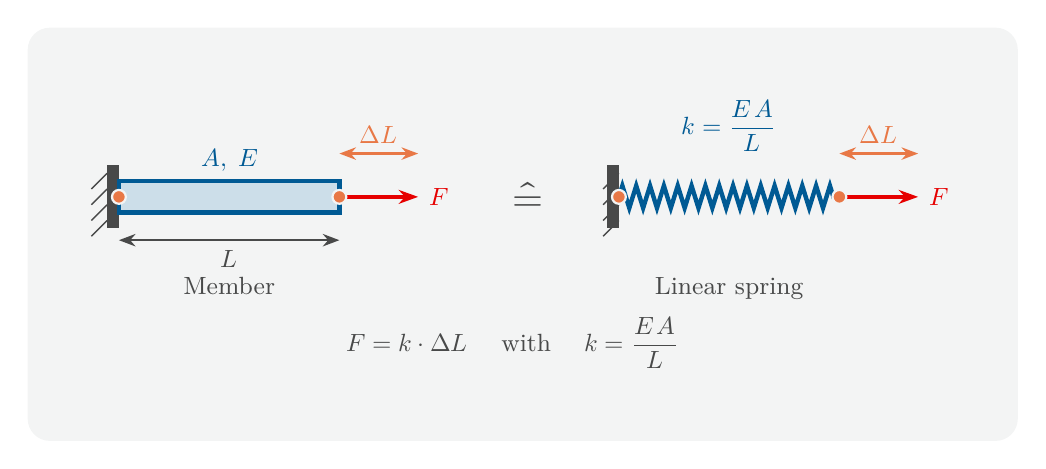
\begin{tikzpicture}[
    show background rectangle,
    background rectangle/.style={fill=my_lightgray, rounded corners=8pt},
    inner frame sep=0.8cm,
    annotation/.style={draw=my_darkgray, thick, -{Stealth[length=7pt, width=5pt]}}
]

    %============================================================
    % LINKE SEITE: Stab
    %============================================================

    % Wandeinspannung links (Stab)
    \fill[my_darkgray] (-0.15, 0.4) rectangle (0.0, -0.4);
    \foreach \y in {0.3, 0.1, -0.1, -0.3} {
        \draw[draw=my_darkgray, line width=0.5pt]
            (-0.15, \y) -- ++(-0.2, -0.2);
    }

    % Stab als Rechteck
    \draw[fill=my_lightblue, draw=my_darkblue, ultra thick]
        (0.0, -0.2) rectangle (2.8, 0.2);

    % Länge L: Doppelpfeil unterhalb des Stabs
    \draw[{Stealth[length=6pt]}-{Stealth[length=6pt]}, draw=my_darkgray, thick]
        (0.0, -0.55) -- (2.8, -0.55)
        node[midway, below, font=\small, text=my_darkgray] {$L$};

    % Querschnitt A: Beschriftung oberhalb
    \node[font=\small, text=my_darkblue, anchor=south]
        at (1.4, 0.2) {$A,\; E$};

    % Kraft F (rechts, nach rechts)
    \draw[draw=my_red, ultra thick, -{Stealth[length=7pt, width=5pt]}]
        (2.8, 0) -- ++(1.0, 0)
        node[anchor=west, font=\small, text=my_red] {$F$};

    % Dehnung ΔL: Doppelpfeil rechts
    \draw[{Stealth[length=6pt]}-{Stealth[length=6pt]}, draw=my_orange, thick]
        (2.8, 0.55) -- (3.8, 0.55)
        node[midway, above, font=\small, text=my_orange] {$\Delta L$};

    % Knotenpunkte
    \draw[fill=my_orange, draw=my_lightgray, thick] (0.0, 0) circle (2.5pt);
    \draw[fill=my_orange, draw=my_lightgray, thick] (2.8, 0) circle (2.5pt);

    % Beschriftung "Stab"
    \node[font=\small, text=my_darkgray, anchor=north]
        at (1.4, -0.9) {Member};

    %============================================================
    % GLEICHHEITSZEICHEN / ENTSPRICHT-ZEICHEN
    %============================================================
    \node[font=\Large, text=my_darkgray] at (5.2, 0) {$\hat{=}$};

    %============================================================
    % RECHTE SEITE: Feder
    %============================================================

    % Wandeinspannung links (Feder)
    \fill[my_darkgray] (6.2, 0.4) rectangle (6.35, -0.4);
    \foreach \y in {0.3, 0.1, -0.1, -0.3} {
        \draw[draw=my_darkgray, line width=0.5pt]
            (6.35, \y) -- ++(-0.2, -0.2);
    }

    % Feder (Zickzack-Dekoration)
    \draw[
        draw=my_darkblue, ultra thick,
        decoration={zigzag, segment length=5pt, amplitude=4pt},
        decorate
    ] (6.35, 0) -- (9.15, 0);

    % Federkonstante k
    \node[font=\small, text=my_darkblue, anchor=south]
        at (7.75, 0.45) {$k = \dfrac{E\,A}{L}$};

    % Kraft F (rechts, nach rechts)
    \draw[draw=my_red, ultra thick, -{Stealth[length=7pt, width=5pt]}]
        (9.15, 0) -- ++(1.0, 0)
        node[anchor=west, font=\small, text=my_red] {$F$};

    % Dehnung ΔL: Doppelpfeil rechts
    \draw[{Stealth[length=6pt]}-{Stealth[length=6pt]}, draw=my_orange, thick]
        (9.15, 0.55) -- (10.15, 0.55)
        node[midway, above, font=\small, text=my_orange] {$\Delta L$};

    % Knotenpunkte
    \draw[fill=my_orange, draw=my_lightgray, thick] (6.35, 0) circle (2.5pt);
    \draw[fill=my_orange, draw=my_lightgray, thick] (9.15, 0) circle (2.5pt);

    % Beschriftung "Feder"
    \node[font=\small, text=my_darkgray, anchor=north]
        at (7.75, -0.9) {Linear spring};

    %============================================================
    % Gleichgewichtsbedingung unten
    %============================================================
    \node[font=\small, text=my_darkgray, anchor=north]
        at (5.0, -1.4) {$F = k \cdot \Delta L \quad$ with $\quad k = \dfrac{E\,A}{L}$};

\end{tikzpicture}
\end{document}